% Options for packages loaded elsewhere
\PassOptionsToPackage{unicode}{hyperref}
\PassOptionsToPackage{hyphens}{url}
\PassOptionsToPackage{dvipsnames,svgnames,x11names}{xcolor}
%
\documentclass[
  10pt,
  ignorenonframetext,
]{beamer}
\usepackage{pgfpages}
\setbeamertemplate{caption}[numbered]
\setbeamertemplate{caption label separator}{: }
\setbeamercolor{caption name}{fg=normal text.fg}
\beamertemplatenavigationsymbolsempty
% Prevent slide breaks in the middle of a paragraph
\widowpenalties 1 10000
\raggedbottom
\setbeamertemplate{part page}{
  \centering
  \begin{beamercolorbox}[sep=16pt,center]{part title}
    \usebeamerfont{part title}\insertpart\par
  \end{beamercolorbox}
}
\setbeamertemplate{section page}{
  \centering
  \begin{beamercolorbox}[sep=12pt,center]{part title}
    \usebeamerfont{section title}\insertsection\par
  \end{beamercolorbox}
}
\setbeamertemplate{subsection page}{
  \centering
  \begin{beamercolorbox}[sep=8pt,center]{part title}
    \usebeamerfont{subsection title}\insertsubsection\par
  \end{beamercolorbox}
}
\AtBeginPart{
  \frame{\partpage}
}
\AtBeginSection{
  \ifbibliography
  \else
    \frame{\sectionpage}
  \fi
}
\AtBeginSubsection{
  \frame{\subsectionpage}
}
\usepackage{amsmath,amssymb}
\usepackage{iftex}
\ifPDFTeX
  \usepackage[T1]{fontenc}
  \usepackage[utf8]{inputenc}
  \usepackage{textcomp} % provide euro and other symbols
\else % if luatex or xetex
  \usepackage{unicode-math} % this also loads fontspec
  \defaultfontfeatures{Scale=MatchLowercase}
  \defaultfontfeatures[\rmfamily]{Ligatures=TeX,Scale=1}
\fi
\usepackage{lmodern}
\usetheme[]{Singapore}
\usefonttheme{serif}
\ifPDFTeX\else
  % xetex/luatex font selection
\fi
% Use upquote if available, for straight quotes in verbatim environments
\IfFileExists{upquote.sty}{\usepackage{upquote}}{}
\IfFileExists{microtype.sty}{% use microtype if available
  \usepackage[]{microtype}
  \UseMicrotypeSet[protrusion]{basicmath} % disable protrusion for tt fonts
}{}
\makeatletter
\@ifundefined{KOMAClassName}{% if non-KOMA class
  \IfFileExists{parskip.sty}{%
    \usepackage{parskip}
  }{% else
    \setlength{\parindent}{0pt}
    \setlength{\parskip}{6pt plus 2pt minus 1pt}}
}{% if KOMA class
  \KOMAoptions{parskip=half}}
\makeatother
\usepackage{xcolor}
\newif\ifbibliography
\usepackage{color}
\usepackage{fancyvrb}
\newcommand{\VerbBar}{|}
\newcommand{\VERB}{\Verb[commandchars=\\\{\}]}
\DefineVerbatimEnvironment{Highlighting}{Verbatim}{commandchars=\\\{\}}
% Add ',fontsize=\small' for more characters per line
\usepackage{framed}
\definecolor{shadecolor}{RGB}{248,248,248}
\newenvironment{Shaded}{\begin{snugshade}}{\end{snugshade}}
\newcommand{\AlertTok}[1]{\textcolor[rgb]{0.94,0.16,0.16}{#1}}
\newcommand{\AnnotationTok}[1]{\textcolor[rgb]{0.56,0.35,0.01}{\textbf{\textit{#1}}}}
\newcommand{\AttributeTok}[1]{\textcolor[rgb]{0.13,0.29,0.53}{#1}}
\newcommand{\BaseNTok}[1]{\textcolor[rgb]{0.00,0.00,0.81}{#1}}
\newcommand{\BuiltInTok}[1]{#1}
\newcommand{\CharTok}[1]{\textcolor[rgb]{0.31,0.60,0.02}{#1}}
\newcommand{\CommentTok}[1]{\textcolor[rgb]{0.56,0.35,0.01}{\textit{#1}}}
\newcommand{\CommentVarTok}[1]{\textcolor[rgb]{0.56,0.35,0.01}{\textbf{\textit{#1}}}}
\newcommand{\ConstantTok}[1]{\textcolor[rgb]{0.56,0.35,0.01}{#1}}
\newcommand{\ControlFlowTok}[1]{\textcolor[rgb]{0.13,0.29,0.53}{\textbf{#1}}}
\newcommand{\DataTypeTok}[1]{\textcolor[rgb]{0.13,0.29,0.53}{#1}}
\newcommand{\DecValTok}[1]{\textcolor[rgb]{0.00,0.00,0.81}{#1}}
\newcommand{\DocumentationTok}[1]{\textcolor[rgb]{0.56,0.35,0.01}{\textbf{\textit{#1}}}}
\newcommand{\ErrorTok}[1]{\textcolor[rgb]{0.64,0.00,0.00}{\textbf{#1}}}
\newcommand{\ExtensionTok}[1]{#1}
\newcommand{\FloatTok}[1]{\textcolor[rgb]{0.00,0.00,0.81}{#1}}
\newcommand{\FunctionTok}[1]{\textcolor[rgb]{0.13,0.29,0.53}{\textbf{#1}}}
\newcommand{\ImportTok}[1]{#1}
\newcommand{\InformationTok}[1]{\textcolor[rgb]{0.56,0.35,0.01}{\textbf{\textit{#1}}}}
\newcommand{\KeywordTok}[1]{\textcolor[rgb]{0.13,0.29,0.53}{\textbf{#1}}}
\newcommand{\NormalTok}[1]{#1}
\newcommand{\OperatorTok}[1]{\textcolor[rgb]{0.81,0.36,0.00}{\textbf{#1}}}
\newcommand{\OtherTok}[1]{\textcolor[rgb]{0.56,0.35,0.01}{#1}}
\newcommand{\PreprocessorTok}[1]{\textcolor[rgb]{0.56,0.35,0.01}{\textit{#1}}}
\newcommand{\RegionMarkerTok}[1]{#1}
\newcommand{\SpecialCharTok}[1]{\textcolor[rgb]{0.81,0.36,0.00}{\textbf{#1}}}
\newcommand{\SpecialStringTok}[1]{\textcolor[rgb]{0.31,0.60,0.02}{#1}}
\newcommand{\StringTok}[1]{\textcolor[rgb]{0.31,0.60,0.02}{#1}}
\newcommand{\VariableTok}[1]{\textcolor[rgb]{0.00,0.00,0.00}{#1}}
\newcommand{\VerbatimStringTok}[1]{\textcolor[rgb]{0.31,0.60,0.02}{#1}}
\newcommand{\WarningTok}[1]{\textcolor[rgb]{0.56,0.35,0.01}{\textbf{\textit{#1}}}}
\usepackage{graphicx}
\makeatletter
\def\maxwidth{\ifdim\Gin@nat@width>\linewidth\linewidth\else\Gin@nat@width\fi}
\def\maxheight{\ifdim\Gin@nat@height>\textheight\textheight\else\Gin@nat@height\fi}
\makeatother
% Scale images if necessary, so that they will not overflow the page
% margins by default, and it is still possible to overwrite the defaults
% using explicit options in \includegraphics[width, height, ...]{}
\setkeys{Gin}{width=\maxwidth,height=\maxheight,keepaspectratio}
% Set default figure placement to htbp
\makeatletter
\def\fps@figure{htbp}
\makeatother
\setlength{\emergencystretch}{3em} % prevent overfull lines
\providecommand{\tightlist}{%
  \setlength{\itemsep}{0pt}\setlength{\parskip}{0pt}}
\setcounter{secnumdepth}{-\maxdimen} % remove section numbering
\newlength{\cslhangindent}
\setlength{\cslhangindent}{1.5em}
\newlength{\csllabelwidth}
\setlength{\csllabelwidth}{3em}
\newlength{\cslentryspacingunit} % times entry-spacing
\setlength{\cslentryspacingunit}{\parskip}
\newenvironment{CSLReferences}[2] % #1 hanging-ident, #2 entry spacing
 {% don't indent paragraphs
  \setlength{\parindent}{0pt}
  % turn on hanging indent if param 1 is 1
  \ifodd #1
  \let\oldpar\par
  \def\par{\hangindent=\cslhangindent\oldpar}
  \fi
  % set entry spacing
  \setlength{\parskip}{#2\cslentryspacingunit}
 }%
 {}
\usepackage{calc}
\newcommand{\CSLBlock}[1]{#1\hfill\break}
\newcommand{\CSLLeftMargin}[1]{\parbox[t]{\csllabelwidth}{#1}}
\newcommand{\CSLRightInline}[1]{\parbox[t]{\linewidth - \csllabelwidth}{#1}\break}
\newcommand{\CSLIndent}[1]{\hspace{\cslhangindent}#1}
\usepackage{multirow}
\setbeamertemplate{navigation symbols}{}
\setbeamertemplate{footline}[page number]
\ifLuaTeX
  \usepackage{selnolig}  % disable illegal ligatures
\fi
\IfFileExists{bookmark.sty}{\usepackage{bookmark}}{\usepackage{hyperref}}
\IfFileExists{xurl.sty}{\usepackage{xurl}}{} % add URL line breaks if available
\urlstyle{same}
\hypersetup{
  pdftitle={Module 9: Boosting and additive trees},
  pdfauthor={Stefanie Muff, Department of Mathematical Sciences, NTNU},
  colorlinks=true,
  linkcolor={Maroon},
  filecolor={Maroon},
  citecolor={Blue},
  urlcolor={blue},
  pdfcreator={LaTeX via pandoc}}

\title{Module 9: Boosting and additive trees}
\subtitle{TMA4268 Statistical Learning V2024}
\author{Stefanie Muff, Department of Mathematical Sciences, NTNU}
\date{March 14 and 15, 2024}

\begin{document}
\frame{\titlepage}

\begin{frame}
\begin{block}{Learning material for this module}
\protect\hypertarget{learning-material-for-this-module}{}
\(~\)

\begin{itemize}
\tightlist
\item
  James et al. (2021): Section 8.2.3 (Boosting)
\end{itemize}

\vspace{2mm}

\begin{itemize}
\tightlist
\item
  Hastie, Tibshirani, and Friedman (2009): The Elements of Statistical
  Learning, Chapter 10
\end{itemize}

\vspace{8mm}

In addition, some material we use is from the book by Boehmke and
Greenwell (2020)

\vspace{2mm}

\begin{itemize}
\tightlist
\item
  \url{https://bradleyboehmke.github.io/HOML/gbm.html}
\end{itemize}
\end{block}
\end{frame}

\begin{frame}
\begin{block}{What will you learn?}
\protect\hypertarget{what-will-you-learn}{}
\(~\)

\begin{itemize}
\tightlist
\item
  Boosting methods -- general terms
\end{itemize}

\vspace{2mm}

\begin{itemize}
\tightlist
\item
  AdaBoost
\end{itemize}

\vspace{2mm}

\begin{itemize}
\tightlist
\item
  Gradient boosting
\end{itemize}

\vspace{2mm}

\begin{itemize}
\tightlist
\item
  Stochastic gradient boosting
\end{itemize}

\vspace{2mm}

\begin{itemize}
\tightlist
\item
  XGBoost: eXtreme Gradient Boosting
\end{itemize}

\vspace{2mm}

\begin{itemize}
\tightlist
\item
  Outlook to modern methods: Light GBM, catboost, ngboost
\end{itemize}

\vspace{2mm}

\begin{itemize}
\tightlist
\item
  Boosting of linear models
\end{itemize}
\end{block}
\end{frame}

\begin{frame}
\begin{block}{Boosting methods}
\protect\hypertarget{boosting-methods}{}
\(~\)

\begin{itemize}
\tightlist
\item
  ``Boosting'' is one of the most powerful learning ideas that is
  currently around.
\end{itemize}

\vspace{2mm}

\begin{itemize}
\tightlist
\item
  First ideas in the 1990s and early 2000s (\emph{e.g.}, Freund and
  Schapire (1997), Ridgeway (1999), J. Friedman, Hastie, and Tibshirani
  (2000))
\end{itemize}

\vspace{2mm}

\begin{itemize}
\tightlist
\item
  Boosting is a general method for building an ensemble out of simpler
  models.
\end{itemize}

\vspace{2mm}

\begin{itemize}
\tightlist
\item
  Boosting is usually applied to models with high bias and low variance,
  usually in the context of boosted regression and classification trees.
\end{itemize}

\vspace{2mm}

\begin{itemize}
\tightlist
\item
  It is also possible to boost, e.g., linear or penalized regression
  models (see presentation by a master student on Friday).
\end{itemize}
\end{block}
\end{frame}

\begin{frame}
\begin{block}{Boosted trees vs deep learning (neural networks)}
\protect\hypertarget{boosted-trees-vs-deep-learning-neural-networks}{}
\(~\)

\begin{itemize}
\tightlist
\item
  Boosted trees and neural networks (deep learning) are currently the
  most powerful competitors in statistical learning.
\end{itemize}

\(~\)

\begin{itemize}
\tightlist
\item
  Kaggle is a website where you find open competitions -- many of them
  are won by tree-based methods.
\end{itemize}

\(~\)

\begin{itemize}
\tightlist
\item
  Maybe you will earn a living from this in the future\ldots? See
  here:\\
  \url{https://www.kaggle.com/competitions}
\end{itemize}
\end{block}
\end{frame}

\begin{frame}
\begin{block}{Examples (recent literature)}
\protect\hypertarget{examples-recent-literature}{}
\centering


\includegraphics[width=0.7\textwidth,height=\textheight]{graphics/trees_vs_nns.png}

\(~\)

\flushleft

From the abstract:

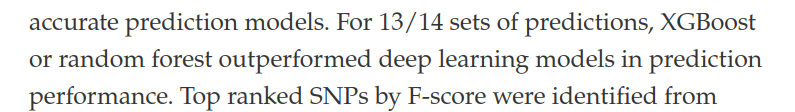
\includegraphics[width=0.8\textwidth,height=\textheight]{graphics/outperform.png}
\end{block}
\end{frame}

\begin{frame}
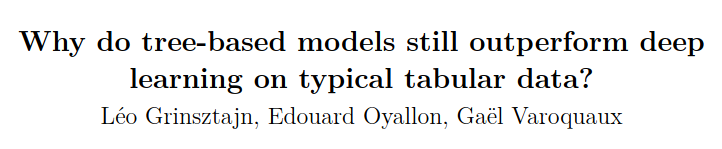
\includegraphics{graphics/why_outperform.png}

See here to access the paper:

\url{https://hal.science/hal-03723551v2}
\end{frame}

\begin{frame}
\begin{block}{Recap: Trees and random forests}
\protect\hypertarget{recap-trees-and-random-forests}{}
\(~\)

\begin{itemize}
\tightlist
\item
  See Module 8: Regression and classification trees.
\end{itemize}

\vspace{2mm}

\begin{itemize}
\tightlist
\item
  Trees are simple, but not very good in predicting.
\end{itemize}

\vspace{2mm}

\begin{itemize}
\tightlist
\item
  Improvements via bagging and random forests.
\end{itemize}

\vspace{2mm}

\begin{itemize}
\tightlist
\item
  Bagging: Build trees on bagged datasets and average over predictions.
\end{itemize}

\vspace{2mm}

\begin{itemize}
\tightlist
\item
  Random forests: Same as bagging, but only use a subset of all
  variables for each new split. Regression: \(p/3\), classification
  \(\sqrt{p}\) of all variables.
\end{itemize}

\vspace{2mm}

\begin{itemize}
\tightlist
\item
  Loss of interpretability is compensated by variable importance
  measures.
\end{itemize}
\end{block}
\end{frame}

\begin{frame}
\begin{block}{Motivation for Boosting in the context of trees}
\protect\hypertarget{motivation-for-boosting-in-the-context-of-trees}{}
\(~\)

\begin{itemize}
\tightlist
\item
  Question: Could we address the shortcomings of single decision trees
  models in some other way than by using random forests?
\end{itemize}

\(~\)

\begin{itemize}
\tightlist
\item
  For example, rather than performing variance reduction on complex
  trees, can we decrease the bias by only using simple trees?
\end{itemize}

\(~\)

\begin{itemize}
\tightlist
\item
  A solution to this problem, making a good model from simple trees, is
  another class of ensemble methods called boosting.
\end{itemize}

\(~\)

\emph{\textcolor{red}{Boosting}} is the process of iteratively adding
basis functions in a greedy fashion so that each additional basis
function further reduces the selected loss function.
\end{block}
\end{frame}

\begin{frame}
\begin{block}{Simple example 1: Boosting for a classification problem:
AdaBoost}
\protect\hypertarget{simple-example-1-boosting-for-a-classification-problem-adaboost}{}
\tiny

Chapter 10.1 in Hastie, Tibshirani, and Friedman (2009), including Fig
10.1 and Algorithm 10.1

\normalsize

\(~\)

\begin{itemize}
\tightlist
\item
  Assume we have a binary classification problem for \(Y\in \{-1,1\}\),
  a vector of predictor variables \(X\), and a classifier \(G(X)\).
\end{itemize}

\vspace{2mm}

\begin{itemize}
\tightlist
\item
  The error rate for a given training sample is then
  \[\text{err} =\frac{1}{N} \sum_{i=1}^N I(y_i \neq G(x_i)) \ .\]
\end{itemize}

\vspace{2mm}

\begin{itemize}
\tightlist
\item
  Here, \(G(X)\) is assumed to be a
  \emph{\textcolor{red}{weak classifier}}, that is, its error rate is
  only \emph{slightly} better than a random guess.
\end{itemize}

\vspace{2mm}

\begin{itemize}
\tightlist
\item
  \(G(X)\) can for example be a tree which is only a ``stump''.
\end{itemize}
\end{block}
\end{frame}

\begin{frame}
\vspace{2mm}

\begin{itemize}
\tightlist
\item
  How would such a weak classifier ever give good predictions?
\end{itemize}

\vspace{2mm}

\begin{itemize}
\tightlist
\item
  Idea:

  \begin{itemize}
  \tightlist
  \item
    Sequentially apply the weak classifier on \emph{modified versions}
    of the data, producing a \emph{sequence} \(G_m(x)\) of weak
    classifiers for \(m=1,2,\ldots,M\).
  \item
    At the end, use a weighted sum
    \(G(x)=\text{sign}\left( \sum_{m=1}^M \alpha_m G_m(x)\right)\) to
    make the final prediction.
  \end{itemize}
\end{itemize}

\vspace{2mm}

\begin{itemize}
\tightlist
\item
  How do we then find the sequence \(G_m(x)\) and the corresponding
  weights \(\alpha_m\)?
\end{itemize}
\end{frame}

\begin{frame}
\centering

\includegraphics[width=0.8\textwidth,height=\textheight]{fig10_1_elements.png}

\small

(Taken from Hastie, Tibshirani, and Friedman (2009) )
\end{frame}

\begin{frame}
\textbf{Algorithm 10.1 (Hastie, Tibshirani, and Friedman (2009)):
AdaBosot.M1}

\(~\)

\begin{enumerate}
\tightlist
\item
  Initialize the observation weights \(w_i= 1/N\), \(i=1,2,\ldots, N\)
\end{enumerate}

\vspace{2mm}

\begin{enumerate}
\setcounter{enumi}{1}
\tightlist
\item
  For \(m=1,2,...,M\):

  \begin{enumerate}
  [a)]
  \tightlist
  \item
    Fit a classifier \(G_m(x)\) to the training data using weights
    \(w_i\).
  \item
    Compute
    \[\text{err}_m = \frac{\sum_{i=1}^N w_i I(y_i\neq G_m(x_i))}{\sum_{i=1}^N w_i} \ .\]
  \item
    Compute \(\alpha_m = \log((1-\text{err}_m)/\text{err}_m)\).
  \item
    Set
    \(w_i \leftarrow w_i \cdot \exp(\alpha_m \cdot I(y_i\neq G_m(x_i)),\)
    \(i=1,2,\ldots, N\).
  \end{enumerate}
\end{enumerate}

\vspace{2mm}

\begin{enumerate}
\setcounter{enumi}{2}
\tightlist
\item
  Output
  \(G(x) = \text{sign}\left[\sum_{m=1}^M \alpha_m G_m(x)\right]\).
\end{enumerate}
\end{frame}

\begin{frame}
Explanations:

\(~\)

\begin{itemize}
\item
  Weights \(\alpha_m\): assigns larger overall weight to good
  classifiers\footnote{Note: When $\text{err}_m<0.5$, then $\alpha_m>0$. Otherwise, the classifier needs to be inverted and $\alpha<0$ makes sense.}.
\item
  Weights \(w_i\) modify the original data. This ensures that
  observations \(i\) with wrong classification in \(G_{m-1}(x)\) obtain
  larger weights, namely \begin{align*} 
   w_i &\leftarrow w_i \cdot \exp(\alpha_m) \ , &\text{ if } y_i \neq G(x_i) \ , \\
   w_i &\leftarrow w_i \ , &\text{ if } y_i = G(x_i) \ .
   \end{align*}
\item
  The sum \(\sum_{m=1}^M \alpha_m G_m(x)\) is a continuous number, so we
  take its sign to get a classification into -1 or 1.
\end{itemize}
\end{frame}

\begin{frame}[fragile]
\begin{block}{Example}
\protect\hypertarget{example}{}
\(~\)

Inspired by (10.2) in the Elements book:

\vspace{2mm}

\begin{itemize}
\tightlist
\item
  Generate features \(X_1, \ldots, X_{10}\) multivariate Gaussian.
\item
  Classify \(y=1\) if \(\sum_{j=1}^{10}X_j^2 > 9.34\), \(y=-1\)
  otherwise.
\item
  1000 traning and 4000 test observations.
\end{itemize}

\(~\)

Yields roughly half/half of each category:

\(~\)

\scriptsize
\centering

\begin{Shaded}
\begin{Highlighting}[]
\FunctionTok{library}\NormalTok{(mvtnorm)}
\FunctionTok{set.seed}\NormalTok{(}\DecValTok{123}\NormalTok{)}
\NormalTok{X }\OtherTok{\textless{}{-}} \FunctionTok{rmvnorm}\NormalTok{(}\DecValTok{5000}\NormalTok{,}\FunctionTok{rep}\NormalTok{(}\DecValTok{0}\NormalTok{,}\DecValTok{10}\NormalTok{))}
\NormalTok{y }\OtherTok{\textless{}{-}} \FunctionTok{ifelse}\NormalTok{(}\FunctionTok{rowSums}\NormalTok{(X}\SpecialCharTok{\^{}}\DecValTok{2}\NormalTok{)}\SpecialCharTok{\textgreater{}}\FloatTok{9.34}\NormalTok{,}\DecValTok{1}\NormalTok{,}\SpecialCharTok{{-}}\DecValTok{1}\NormalTok{)}
\FunctionTok{hist}\NormalTok{(y,}\AttributeTok{title=}\StringTok{""}\NormalTok{)}
\end{Highlighting}
\end{Shaded}

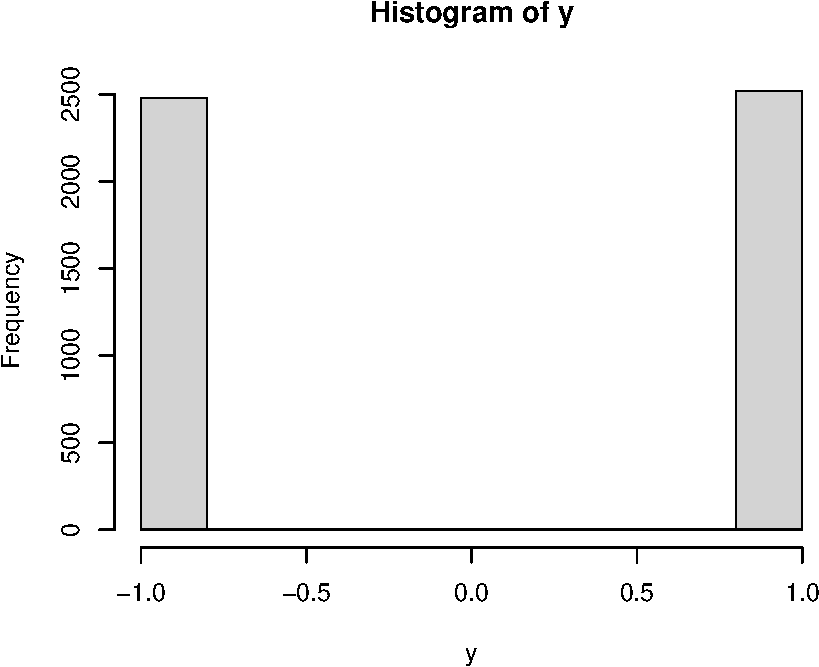
\includegraphics[width=0.4\linewidth]{9TreeBoosting_files/figure-beamer/unnamed-chunk-1-1}
\end{block}
\end{frame}

\begin{frame}[fragile]
Fit AdaBoost on the training data using the function \texttt{ada()} from
the \texttt{ada} R package. The function uses classification trees as
weak learners. We use default choice for tree depth (tree depth is
decided on a case-by-case basis):

\vspace{2mm}

\scriptsize
\centering

\begin{Shaded}
\begin{Highlighting}[]
\FunctionTok{library}\NormalTok{(ada)}
\NormalTok{dd }\OtherTok{\textless{}{-}} \FunctionTok{data.frame}\NormalTok{(X,y)}
\NormalTok{dd.train }\OtherTok{\textless{}{-}}\NormalTok{ dd[}\DecValTok{1}\SpecialCharTok{:}\DecValTok{1000}\NormalTok{,]}
\NormalTok{dd.test }\OtherTok{\textless{}{-}}\NormalTok{ dd[}\DecValTok{1001}\SpecialCharTok{:}\DecValTok{5000}\NormalTok{,]}

\FunctionTok{set.seed}\NormalTok{(}\DecValTok{4268}\NormalTok{)}
\NormalTok{r.ada }\OtherTok{\textless{}{-}} \FunctionTok{ada}\NormalTok{(y}\SpecialCharTok{\textasciitilde{}}\NormalTok{.,dd.train,}\AttributeTok{iter=}\DecValTok{400}\NormalTok{,}\AttributeTok{type=}\StringTok{"discrete"}\NormalTok{, }\AttributeTok{loss=}\StringTok{"ada"}\NormalTok{, }\AttributeTok{control=}\FunctionTok{rpart.control}\NormalTok{())}
\FunctionTok{plot}\NormalTok{(r.ada)}
\end{Highlighting}
\end{Shaded}

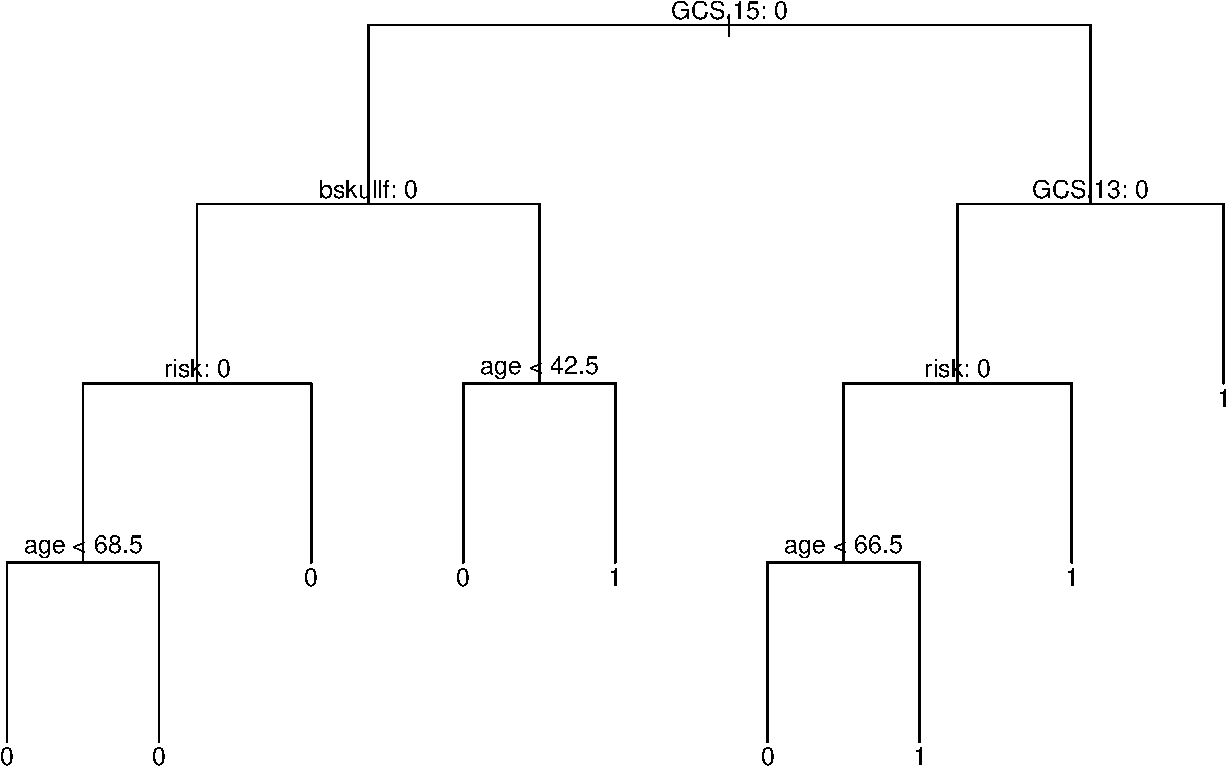
\includegraphics[width=0.5\linewidth]{9TreeBoosting_files/figure-beamer/unnamed-chunk-2-1}
\end{frame}

\begin{frame}[fragile]
\begin{block}{Error rates: AdaBoost vs random forest}
\protect\hypertarget{error-rates-adaboost-vs-random-forest}{}
\(~\)

AdaBoost test error:

\vspace{2mm}

\scriptsize

\begin{Shaded}
\begin{Highlighting}[]
\NormalTok{ada.pred }\OtherTok{\textless{}{-}} \FunctionTok{predict}\NormalTok{(r.ada,dd.test)}
\FunctionTok{sum}\NormalTok{(dd.test}\SpecialCharTok{$}\NormalTok{y}\SpecialCharTok{!=}\NormalTok{ada.pred)}\SpecialCharTok{/}\DecValTok{4000}
\end{Highlighting}
\end{Shaded}

\begin{verbatim}
## [1] 0.099
\end{verbatim}

\(~\)

\(~\)

\normalsize

Random forest test error:

\vspace{2mm}

\scriptsize

\begin{Shaded}
\begin{Highlighting}[]
\FunctionTok{library}\NormalTok{(randomForest)}
\FunctionTok{set.seed}\NormalTok{(}\DecValTok{123}\NormalTok{)}
\NormalTok{rf.boston}\OtherTok{=}\FunctionTok{randomForest}\NormalTok{(}\FunctionTok{as.factor}\NormalTok{(y)}\SpecialCharTok{\textasciitilde{}}\NormalTok{.,dd.train,}\AttributeTok{mtry=}\DecValTok{3}\NormalTok{,}
                       \AttributeTok{ntree=}\DecValTok{1000}\NormalTok{)}
\NormalTok{rf.pred }\OtherTok{\textless{}{-}} \FunctionTok{predict}\NormalTok{(rf.boston,}\AttributeTok{newdata=}\NormalTok{dd.test)}
\FunctionTok{sum}\NormalTok{(dd.test}\SpecialCharTok{$}\NormalTok{y}\SpecialCharTok{!=}\NormalTok{rf.pred)}\SpecialCharTok{/}\DecValTok{4000}
\end{Highlighting}
\end{Shaded}

\begin{verbatim}
## [1] 0.17425
\end{verbatim}
\end{block}
\end{frame}

\begin{frame}{Simple example 2: Boosting regression trees}
\protect\hypertarget{simple-example-2-boosting-regression-trees}{}
\(~\)

In tree boosting, trees are grown \emph{sequentially} so that each tree
is grown using information from the previous tree.

\vspace{2mm}

\begin{enumerate}
\tightlist
\item
  Build a decision tree with \(d\) splits (and \(d+1\) terminal notes).
\item
  Improve the model in areas where the model didn't perform well. This
  is done by fitting a decision tree to the \emph{residuals of the
  model}. This procedure is called \emph{learning slowly}.
\item
  The first decision tree is then updated based on the residual tree,
  but with a weight.
\end{enumerate}

The procedure is repeated until some stopping criterion is reached. Each
of the trees can be very small, with just a few terminal nodes (or just
one split).
\end{frame}

\begin{frame}
\textbf{Algorithm 8.2: Boosting for regression trees}

\begin{enumerate}
\tightlist
\item
  Set \(\hat{f}(x) = 0\) and \(r_i = y_i\) for all \(i\) in the training
  set.
\item
  For \(b=1,2,...,B\), repeat:

  \begin{enumerate}
  [a)]
  \tightlist
  \item
    Fit a tree \(\hat{f}^b\) with \(d\) splits (\(d+1\) terminal nodes)
    to the training data.\\
  \item
    Update \(\hat{f}\) by adding in a shrunken version of the new tree:
    \[\hat{f}(x) \leftarrow \hat{f}(x)+\nu \hat{f}^b(x).\]\\
  \item
    Update the residuals, \[r_i \leftarrow r_i - \nu \hat{f}^b(x_i).\]\\
  \end{enumerate}
\item
  The boosted model is \(\hat{f}(x) = \sum_{b=1}^B \nu \hat{f}^b(x).\)
\end{enumerate}

Boosting has three tuning parameters which need to be set (\(B\),
\(\nu\), \(d\)), and can be found using cross-validation.
\end{frame}

\begin{frame}
\textbf{Tuning parameters}

\begin{itemize}
\item
  \textbf{Number of trees \(B\)}. Could be chosen using
  cross-validation. A too small value of \(B\) would imply that much
  information is unused (remember that boosting is a slow learner),
  whereas a too large value of \(B\) may lead to overfitting.
\item
  \textbf{Shrinkage parameter \(\nu\)}. Controls the rate at which
  boosting learns. \(\nu\) scales the new information from the \(b\)-th
  tree, when added to the existing tree \(\hat{f}\). Choosing a small
  value for \(\nu\) ensures that the algorithm learns slowly, but will
  require a larger \(B\). Typical values of \(\nu\) is 0.1 or 0.01.
\item
  \textbf{Interaction depth \(d\)}: The number of splits in each tree.
  This parameter controls the complexity of the boosted tree ensemble
  (the level of interaction between variables that we may estimate). By
  choosing \(d=1\) a tree stump will be fitted at each step and this
  gives an additive model.
\end{itemize}
\end{frame}

\begin{frame}
A very simple illustration of this idea can be found here:

\url{https://arogozhnikov.github.io/2016/06/24/gradient_boosting_explained.html}
\end{frame}

\begin{frame}[fragile]
\begin{block}{Revisit the Boston data from module 8}
\protect\hypertarget{revisit-the-boston-data-from-module-8}{}
\(~\)

We are now finally boosting the Boston trees! We use the \texttt{gbm()}
function from the respective R package. We boost with 5000 trees and
allow the interaction depth (number of splits per tree) to be of degree
4:

\vspace{2mm}

\scriptsize

\begin{Shaded}
\begin{Highlighting}[]
\FunctionTok{library}\NormalTok{(gbm)}
\FunctionTok{set.seed}\NormalTok{(}\DecValTok{1}\NormalTok{)}
\NormalTok{boost.boston}\OtherTok{=}\FunctionTok{gbm}\NormalTok{(medv}\SpecialCharTok{\textasciitilde{}}\NormalTok{.,}\AttributeTok{data=}\NormalTok{Boston[train,],}
                 \AttributeTok{distribution=}\StringTok{"gaussian"}\NormalTok{,}
                 \AttributeTok{n.trees=}\DecValTok{5000}\NormalTok{,}\AttributeTok{interaction.depth=}\DecValTok{4}\NormalTok{)}
\FunctionTok{summary}\NormalTok{(boost.boston,}\AttributeTok{plotit=}\ConstantTok{FALSE}\NormalTok{)}
\end{Highlighting}
\end{Shaded}

\begin{verbatim}
##             var    rel.inf
## rm           rm 43.9919329
## lstat     lstat 33.1216941
## crim       crim  4.2604167
## dis         dis  4.0111090
## nox         nox  3.4353017
## black     black  2.8267554
## age         age  2.6113938
## ptratio ptratio  2.5403035
## tax         tax  1.4565654
## indus     indus  0.8008740
## rad         rad  0.6546400
## zn           zn  0.1446149
## chas       chas  0.1443986
\end{verbatim}
\end{block}
\end{frame}

\begin{frame}[fragile]
\textbf{Prediction on the test set}

\begin{itemize}
\item
  Calculate the MSE on the test set, first for the model with
  \(\nu=0.001\) (default), then with \(\nu=0.2\).
\item
  Ideally, we should do a cross-validation to find the best \(\nu\) over
  a grid (comes later), but here it seems not to make a big difference.
\end{itemize}

\(~\)

\scriptsize

\begin{Shaded}
\begin{Highlighting}[]
\NormalTok{yhat.boost}\OtherTok{=}\FunctionTok{predict}\NormalTok{(boost.boston,}\AttributeTok{newdata=}\NormalTok{Boston[}\SpecialCharTok{{-}}\NormalTok{train,],}\AttributeTok{n.trees=}\DecValTok{5000}\NormalTok{)}
\FunctionTok{mean}\NormalTok{((yhat.boost}\SpecialCharTok{{-}}\NormalTok{boston.test)}\SpecialCharTok{\^{}}\DecValTok{2}\NormalTok{)}
\end{Highlighting}
\end{Shaded}

\begin{verbatim}
## [1] 18.84709
\end{verbatim}

\vspace{2mm}

\begin{Shaded}
\begin{Highlighting}[]
\NormalTok{boost.boston}\OtherTok{=}\FunctionTok{gbm}\NormalTok{(medv}\SpecialCharTok{\textasciitilde{}}\NormalTok{.,}\AttributeTok{data=}\NormalTok{Boston[train,],}\AttributeTok{distribution=}\StringTok{"gaussian"}\NormalTok{,}
                 \AttributeTok{n.trees=}\DecValTok{5000}\NormalTok{,}\AttributeTok{interaction.depth=}\DecValTok{4}\NormalTok{,}\AttributeTok{shrinkage=}\FloatTok{0.2}\NormalTok{,}\AttributeTok{verbose=}\NormalTok{F)}
\NormalTok{yhat.boost}\OtherTok{=}\FunctionTok{predict}\NormalTok{(boost.boston,}\AttributeTok{newdata=}\NormalTok{Boston[}\SpecialCharTok{{-}}\NormalTok{train,],}\AttributeTok{n.trees=}\DecValTok{5000}\NormalTok{)}
\FunctionTok{mean}\NormalTok{((yhat.boost}\SpecialCharTok{{-}}\NormalTok{boston.test)}\SpecialCharTok{\^{}}\DecValTok{2}\NormalTok{)}
\end{Highlighting}
\end{Shaded}

\begin{verbatim}
## [1] 18.33455
\end{verbatim}
\end{frame}

\begin{frame}{Boosting more generally}
\protect\hypertarget{boosting-more-generally}{}
\(~\)

\begin{itemize}
\tightlist
\item
  AdaBoost.M1 and the above regression tree example are both relatively
  simple special cases of (tree) boosting.
\end{itemize}

\vspace{2mm}

\begin{itemize}
\tightlist
\item
  We therefore step a bit back and look at boosting methods in more
  generality.
\end{itemize}

\vspace{2mm}

\begin{itemize}
\tightlist
\item
  In general terms, we are looking for expansions that take the form
  \[f(x) = \sum_{m=1}^M \beta_m b(\mathbf{x};\gamma) \ , \] where
  \(b(\mathbf{x};\gamma)\) are (simple) \emph{basis functions} in
  \(\mathbf{x}\) characterized by a set of parameters \(\gamma\), and
  \(\beta_m\) are the corresponding expansion coefficients.
\end{itemize}

\vspace{2mm}

\begin{itemize}
\tightlist
\item
  In the following, we focus on the case where \(b(\mathbf{x};\gamma)\)
  correspond to trees.
\end{itemize}
\end{frame}

\begin{frame}
\begin{block}{Boosting trees -- what do we want to minimize?}
\protect\hypertarget{boosting-trees-what-do-we-want-to-minimize}{}
\(~\)

Start by looking again at \emph{a single tree}. We need to find regions
\(R_j\) and values \(f(x)=\gamma_j\) if \(x\in R_j\), for
\(j=1,2,\ldots,J\). The tree can then be expressed as

\[T(x;\Theta) = \sum_{j=1}^J \gamma_j I(x\in R_j) \ .\] \(~\)

Formally we want to minimize

\begin{equation}\label{eq:treeopt}
\hat\Theta = \arg \min_\Theta \sum_{j=1}^J \sum_{x_i \in R_j} L(y_i,\gamma_i) \ , 
\end{equation} for a set of observations \((x_i,y_i)\)
\((i=1,\ldots,N)\) and for loss function \(L()\), for example
squared-error, Gini, deviance loss etc.
\end{block}
\end{frame}

\begin{frame}
\label{sl:regions}

The optimization problem is split into two parts:

\(~\)

\begin{enumerate}
[1)]
\tightlist
\item
  \textbf{Find \(\gamma_j\) given \(R_j\)}: Given \(R_j\), estimating
  \(\gamma_j\) is easy. Either \(\gamma_j=\overline{y_j}\) or majority
  vote for classification.
\end{enumerate}

\vspace{2mm}

\begin{enumerate}
[1)]
\setcounter{enumi}{1}
\tightlist
\item
  \textbf{Finding the regions \(R_j\)}: This is the hard part. Usually
  approximative via a greedy algorithm. Often, use smoother
  approximations of the optimization criterion
  \begin{equation}\label{eq:approx}
  \tilde\Theta = \arg \min_\Theta \sum_{j=1}^J \sum_{x_i \in R_j} \tilde{L}(y_i,T(x_i,\Theta)) \ , 
  \end{equation} and then use \(\hat{R}_j=\tilde{R}_j\) to find
  \(\gamma_j\) using the original criterion \eqref{eq:treeopt}.
\end{enumerate}
\end{frame}

\begin{frame}
\begin{block}{From single trees to boosting}
\protect\hypertarget{from-single-trees-to-boosting}{}
\label{sl:toBoosting}

\(~\)

\begin{itemize}
\tightlist
\item
  Previous slide summarizes how to find \emph{one tree}.
\end{itemize}

\vspace{2mm}

\begin{itemize}
\item
  The result of boosting is a \emph{sum of \(M\) trees}
  \[f_M(x) = \sum_{m=1}^M T(x;\Theta_m) \ .\] \vspace{2mm}
\item
  Tree boosting is about \emph{how to find each tree}.
\end{itemize}

\vspace{2mm}

\begin{itemize}
\tightlist
\item
  At each step, one must solve \begin{equation}\label{eq:boosted}
  \hat\Theta_m = \arg \min_{\Theta_m} \sum_{i=1}^N L\left(y_i, f_{m-1}(x_i) + T(x_i;\Theta_m)\right) 
  \end{equation} to find the next set \(\Theta_m\), given
  \(f_{m-1}(x)\).
\end{itemize}
\end{block}
\end{frame}

\begin{frame}
\(~\)

\begin{itemize}
\tightlist
\item
  For a \emph{\textcolor{red}{regression tree}} with
  \textbf{squared-error loss}, solving \eqref{eq:boosted} is the same as
  for a single tree. Just sequentially fit regression trees to the
  residuals \(r_i = y_i - f(x_i)\) from the previous tree.
\end{itemize}

\(~\)

\begin{itemize}
\tightlist
\item
  For \emph{\textcolor{red}{binary classification}} with
  \(Y\in \{-1,1\}\) and \textbf{exponential loss}
  \[L(y,f(x))=\exp(-yf(x)) \ ,\] we get AdaBoost (Algorithm 10.1).
\end{itemize}

\(~\)
\end{frame}

\begin{frame}
\(~\)

\begin{itemize}
\tightlist
\item
  Both strategies on the previous slide are straightforward, but
  \emph{not very robust}.
\end{itemize}

\vspace{2mm}

\begin{itemize}
\tightlist
\item
  We therefore look for general algorithms that can use any loss
  function \(L(f)\) when \(f\) is \textbf{contrained to be a sum of
  trees}.
\end{itemize}

\vspace{2mm}

\begin{itemize}
\tightlist
\item
  It is then sometimes better to approximate the loss function as
  \(\tilde{L}(f)\) in the tree-building step (step \eqref{eq:approx} on
  slide \ref{sl:regions}) and use \(L(f)\) only to determine the
  \(\gamma_{jm}\) values in each tree \(m\).
\end{itemize}

\(~\)

\textbf{Main idea:} Iteratively build trees for the \emph{gradient} of
the previous tree. Motivated by steepest descent.
\end{frame}

\begin{frame}
\begin{block}{Steepest descent -- a numerical optimization technique}
\protect\hypertarget{steepest-descent-a-numerical-optimization-technique}{}
\(~\)

\begin{itemize}
\tightlist
\item
  \emph{\textcolor{red}{Steepest descent}} is a \emph{general} numerical
  optimization technique.
\end{itemize}

\vspace{2mm}

\begin{itemize}
\tightlist
\item
  When trying to find the best function \(f(x)\) that minimizes a loss
  function \[L(f) = \sum_{i=1}^N L(y_i,f(x_i)) \ ,\] the direction of
  steepest descent is given by an \(n\)-dimensional vector with entries
  \[g_{i} = \left[ \frac{\partial L(y_i,f(x_i))}{\partial f(x_i)} \right] \ ,\]
  with gradient vector
  \(\mathbf{g}^\top = (g_{1},g_{2},\ldots, g_{N})\).
\end{itemize}
\end{block}
\end{frame}

\begin{frame}
\begin{itemize}
\tightlist
\item
  If we repeat this iteratively, we can denote the gradient at step
  \(m\) as \(\mathbf{g}_m^\top = (g_{1m},g_{2m},\ldots, g_{Nm})\).
\end{itemize}

\vspace{2mm}

\begin{itemize}
\tightlist
\item
  To update from \(\mathbf{f}_{m-1}\) to
  \(\mathbf{f}_m\)\footnote{$\mathbf{f}_m = (f_m(x_1),f_m(x_2),\ldots, f_m(x_N))^\top$ },
  we search for the largest decrease in the loss function as
\end{itemize}

\[\rho_m = \arg \min_\rho L(\mathbf{f}_{m-1} - \rho \mathbf{g}_m) \ , \]

\(~\)

\begin{itemize}
\tightlist
\item
  Then update \(\mathbf{f}_m = \mathbf{f}_{m-1} - \rho_m \mathbf{g}_m\).
\end{itemize}

\(~\)

\pause

\begin{itemize}
\tightlist
\item
  However, recall that we want to fit trees
  \(f_m(x)=T(x;\Theta_m)=\sum_{j=1}^J \gamma_j I(x\in R_j)\), not
  aribtrary predictor functions \(\mathbf{f}_m\).
\end{itemize}
\end{frame}

\begin{frame}
\begin{block}{Gradient Boosting: Steepest descent for trees}
\protect\hypertarget{gradient-boosting-steepest-descent-for-trees}{}
\(~\)

\textbf{The central idea}: find a tree \(T(x;\Theta_m)\) that is as
close as possible to the negative gradient

\begin{equation}
\tilde{\Theta}_m= \arg \min_\Theta \sum_{i=1}^N (-g_{im} -T(x_i;\Theta))^2 \ .
\end{equation}

\vspace{8mm}

That is: Fit a tree \(T\) to the negative gradient using least squares!
\end{block}
\end{frame}

\begin{frame}
\vspace{2mm}

\begin{itemize}
\tightlist
\item
  This leads to regions \(\tilde{R}_{jm}\) that are close (enough) to
  the optimal regions \(R_{jm}\) from equation \eqref{eq:boosted} on
  slide \eqref{sl:toBoosting}.\\
  \vspace{2mm} \(\rightarrow\) This corresponds to the step to find the
  regions \(\hat{R}_{jm}=\tilde{R}_{jm}\) (step 2 on slide
  \ref{sl:regions}).
\end{itemize}

\(~\)

\begin{itemize}
\tightlist
\item
  Finally, find \(\gamma_{jm}\) given the regions \(\hat{R}_{jm}\).\\
  \vspace{2mm} \(\rightarrow\) This is the ``easy'' step 1 on slide
  \ref{sl:regions} and is done by \begin{equation*}
  \hat\gamma_{jm} = \arg \min_{\gamma} \sum_{x_i \in \hat{R}_{jm}} L(y_i, f_{m-1}(x_i) + \gamma) \ .
  \end{equation*}
\end{itemize}
\end{frame}

\begin{frame}
\begin{block}{Gradient tree boosting algorithm}
\protect\hypertarget{gradient-tree-boosting-algorithm}{}
\(~\)

\textbf{Algorithm 10.3} in Hastie, Tibshirani, and Friedman (2009):

\(~\)

\begin{enumerate}
\tightlist
\item
  Initialize \(f_0(x) = \arg \min_\gamma \sum_{i=1}^N L(y_i,\gamma)\).
\end{enumerate}

\vspace{1mm}

\begin{enumerate}
\setcounter{enumi}{1}
\item
  For \(m=1\) to \(M\):

  \begin{enumerate}
  [(a)]
  \tightlist
  \item
    For \(i=1,2,\ldots, N\) compute
    \[r_{im} = - \left[ \frac{\partial L(y_i,f(x_i))}{\partial f(x_i)} \right] \ .\]
  \item
    Fit a regression tree to the targets \(r_{im}\), giving terminal
    regions \(R_{jm}, j=1,2,\ldots , J_m\).
  \end{enumerate}

  \vspace{1mm}

  \begin{enumerate}
  [(a)]
  \setcounter{enumii}{2}
  \item
    For \(j=1,2,\ldots, J_m\) compute
    \[\gamma_{jm} = \arg \min_\gamma \sum_{x_i \in R_{jm}} L(y_i, f_{m-1}(x_i) + \gamma) \ .\]
    \vspace{1mm}
  \item
    Update
    \(f_m(x)=f_{m-1}(x) + \sum_{j=1}^{J_m} \gamma_{jm}I(x\in R_{jm})\).
  \end{enumerate}
\end{enumerate}

\vspace{1mm}

\begin{enumerate}
\setcounter{enumi}{2}
\tightlist
\item
  Output \(\hat{f}(x)=f_M(x)\).
\end{enumerate}
\end{block}
\end{frame}

\begin{frame}
\begin{block}{Gradient tree boosting for regression}
\protect\hypertarget{gradient-tree-boosting-for-regression}{}
\(~\)

\(r_{im} = - \left[ \frac{\partial L(y_i,f(x_i))}{\partial f(x_i)} \right]\)
are the components of the negative gradient. We call them
\emph{\textcolor{red}{generalized}} or
\emph{\textcolor{red}{pseudo-residuals}}. Why?

\vspace{8mm}

\begin{itemize}
\tightlist
\item
  Look at the (scaled) \textbf{quadratic loss function}
  \[L(y_i,f(x_i)) = \frac{1}{2} (y_i-f(x_i))^2.\]
\end{itemize}

\vspace{2mm}

\begin{itemize}
\tightlist
\item
  Then \[-\partial L(y_i,f(x_i))/\partial f(x_i) = y_i - f(x_i) \ , \]
  which is the residual.
\end{itemize}

\vspace{2mm}

\begin{itemize}
\tightlist
\item
  Gradient boosting is thus equivalent to reducing the quadratic loss
  function as fast as possible (``steepest descent'').
\end{itemize}

\vspace{2mm}

\begin{itemize}
\tightlist
\item
  However: Gradient boosting works for \emph{any loss function}.
\end{itemize}
\end{block}
\end{frame}

\begin{frame}
\begin{block}{Gradient tree boosting for regression -- loss functions}
\protect\hypertarget{gradient-tree-boosting-for-regression-loss-functions}{}
\(~\)

\begin{itemize}
\tightlist
\item
  \textbf{Quadratic loss}: Previous slide. Not very robust -- a lot of
  weight on extreme observations.
\end{itemize}

\vspace{8mm}

Popular alternatives:

\vspace{2mm}

\begin{itemize}
\tightlist
\item
  \textbf{Absolute loss}: \[L(y,f(x)) = |y-f(x)| \]
\end{itemize}

\vspace{2mm}

\begin{itemize}
\tightlist
\item
  \textbf{Huber loss}: \[L(y,f(x)) = \begin{cases}
   (y-f(x))^2 &  \text{ for }  |y-f(x)|\leq \delta \ ,\\
  2\delta |y-f(x)| -\delta^2 &  \text{ otherwise.} 
  \end{cases}
  \]
\end{itemize}
\end{block}
\end{frame}

\begin{frame}
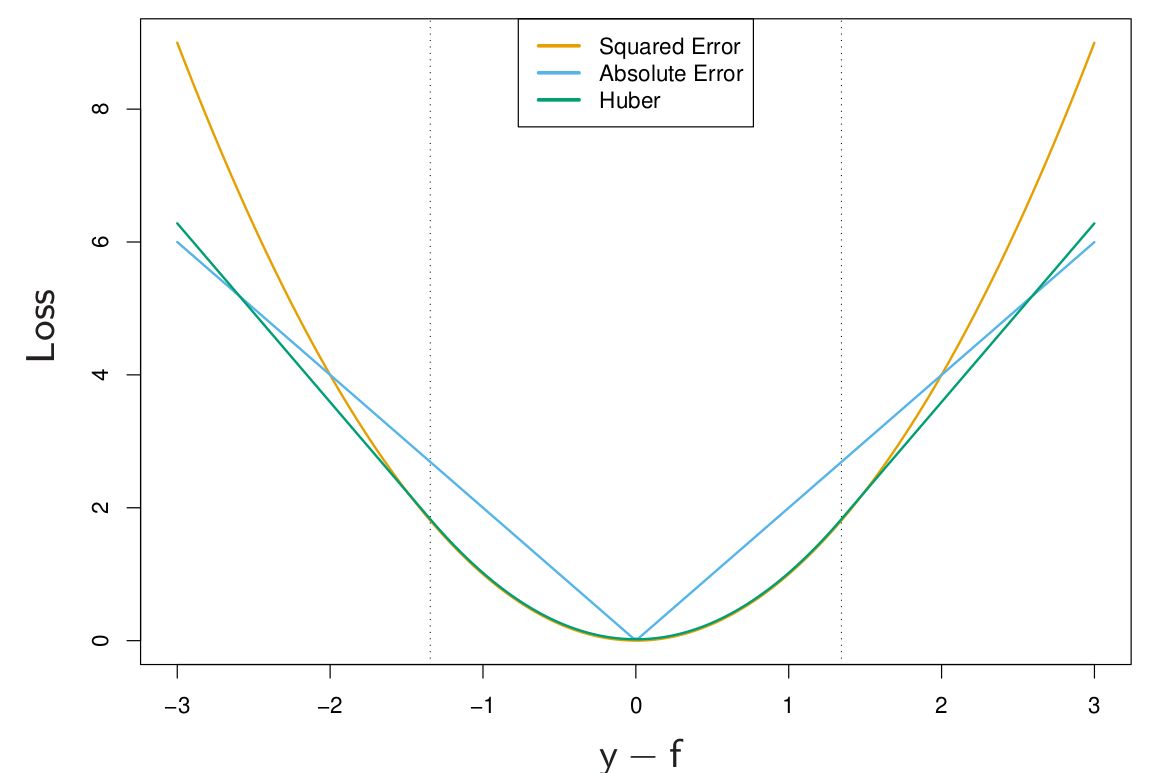
\includegraphics{graphics/robust_loss.png}
\end{frame}

\begin{frame}
\begin{block}{Gradient tree boosting for binary classification}
\protect\hypertarget{gradient-tree-boosting-for-binary-classification}{}
\(~\)

Replace the squared error loss by the \emph{binomial deviance} (now with
\(y\in \{0,1\}\)):

\[L(y,f(x)) = -I(y=1) \log(p(x)) - I(y=0) \log(1-p(x)) \ , \] with
\[p(x) = \frac{e^{f(x)}}{1+e^{f(x)}} \ .\]

\(~\)

Here, \(f(x)\) is the (linear) predictor function encoding the tree
ensemble, similar to logistic regression.

\(~\)
\end{block}
\end{frame}

\begin{frame}
\begin{block}{Gradient tree boosting for classification into \(K\)
classes}
\protect\hypertarget{gradient-tree-boosting-for-classification-into-k-classes}{}
\(~\)

For \(K>2\) classes, use as loss function the
\emph{\textcolor{red}{K-class multinomial deviance}}

\begin{align}
L(y,f(x)) &= -\sum_{k=1}^K I(y = k) \log (p_k(x)) \\ 
 & = -\sum_{k=1}^K I(y = k) f_k(x) + \log(\sum_{l=1}^K e^{f_l(x)}) \ ,
 \end{align}

with class probabilities
\[p_k(x) = \frac{e^{f_k(x)}}{\sum_{l=1}^K e^{f_l(x)}} \ , \] and
corresponding functions \(f(x)\).
\end{block}
\end{frame}

\begin{frame}
\(~\)

\begin{itemize}
\item
  Plugging \(p_k(x)\) into the multinomial deviance, we see that\\
  \[-g_{ikm} = \left[ \frac{\partial L(y_i, f_1(x_i),\ldots, f_K(x_i))}{\partial f_k(x_i)} \right]_{f_{m-1}(x_i)} = I(y_i =k) - p_k(x_i) \ .\]
  \(~\)
\item
  For \(K\) classes, we must build \(K\) trees in each iteration of step
  2. in the boosting procedure!
\end{itemize}

\vspace{2mm}

\begin{itemize}
\tightlist
\item
  In step 3., we aggregate the class probabilities for each class \(k\).
\end{itemize}
\end{frame}

\begin{frame}{Practical considerations}
\protect\hypertarget{practical-considerations}{}
The three main ingredients of gradient boosting, which we need to
determine in practice:

\vspace{2mm}

\begin{itemize}
\item
  \emph{\textcolor{red}{Weak Learner}}: A weak learner is one that
  classifies our data but does so poorly, perhaps no better than random
  guessing. In other words, it has a high error rate. These are
  typically decision trees (also called decision stumps, because they
  are less complicated than typical decision trees).
\item
  \emph{\textcolor{red}{Additive Model}}: This is the iterative and
  sequential approach of adding the trees (weak learners) one step at a
  time. After each iteration, we need to be closer to our final model,
  since each iteration should reduce the value of our loss function.
\item
  \emph{\textcolor{red}{Loss Function}}: The function we want to
  minimize. Its role is to estimate how good the model is at making
  predictions with the given data.
\end{itemize}
\end{frame}

\begin{frame}{Parameter tuning}
\protect\hypertarget{parameter-tuning}{}
\(~\)

Given a loss function, we can tune the following parameters:

\(~\)

\textbf{Tree hyperparameters (weak learner):}

\begin{enumerate}
[a)]
\item
  Tree size (depth) in each iteration
\item
  Minimum observations in terminal nodes
\end{enumerate}

\(~\)

\textbf{Boosting hyperparameters (additive model):}

\begin{enumerate}
[a)]
\setcounter{enumi}{2}
\item
  Number of trees \(M\), i.e., the number of boosting iterations
\item
  The learning rate \(\nu\)
\end{enumerate}
\end{frame}

\begin{frame}
\begin{block}{a) Finding the right tree depth in boosting}
\protect\hypertarget{a-finding-the-right-tree-depth-in-boosting}{}
(10.11 in the Elements book)

\(~\)

\begin{itemize}
\tightlist
\item
  Historically, large trees were grown, followed by pruning, in each
  iteration of the boosting process.
\end{itemize}

\vspace{2mm}

\begin{itemize}
\tightlist
\item
  However, this assumes that each tree is the last one in the algorithm
  (why?).
\end{itemize}

\vspace{2mm}

\begin{itemize}
\tightlist
\item
  Better strategy: All trees are the same size.
\end{itemize}

\pause

\vspace{6mm}

Given that \(J\) is the number of leaves (\(J-\)terminal node tree):

\vspace{2mm}

\begin{itemize}
\tightlist
\item
  \textbf{which size should we then choose?}
\item
  \textbf{Why?}
\end{itemize}

\vspace{2mm}

Discuss!
\end{block}
\end{frame}

\begin{frame}
Some considerations / drawings:

\vspace{60mm}

\(~\)

In the end, \(J\) is a tuning parameters, but does usually not give much
better results than when using \(J\approx 4 \text{ to } 6\).

\vspace{50mm}
\end{frame}

\begin{frame}
\begin{block}{b) Minimum number of observations in terminal nodes}
\protect\hypertarget{b-minimum-number-of-observations-in-terminal-nodes}{}
\(~\)

\begin{itemize}
\tightlist
\item
  This hyper-parameter is less relevant for large data sets.
\end{itemize}

\vspace{2mm}

\begin{itemize}
\tightlist
\item
  Moreover, by giving tree depth and tuning the number of trees, we can
  hope to get this parameter ``for free''.
\end{itemize}

\vspace{2mm}

\begin{itemize}
\tightlist
\item
  A reason to care anyway is that larger number of observations per leaf
  are needed to get a good mean estimates.
\end{itemize}

\(~\)

\(~\)
\end{block}
\end{frame}

\begin{frame}
\begin{block}{c) The number of trees (regularization strategy 1)}
\protect\hypertarget{c-the-number-of-trees-regularization-strategy-1}{}
\(~\)

\begin{itemize}
\tightlist
\item
  When the number of trees \(M\) is growing, the training error is
  reduced.
\end{itemize}

\vspace{2mm}

\begin{itemize}
\tightlist
\item
  For too large \(M\), we will overfit the training data.
\end{itemize}

\vspace{2mm}

\begin{itemize}
\tightlist
\item
  Therefore, need to monitor prediction error on a validation sample and
  do ``early stopping''.
\end{itemize}

\vspace{2mm}

\begin{itemize}
\tightlist
\item
  Alternative: Cross-validation
\end{itemize}

\vspace{6mm}

\(\rightarrow\) \(M\) is a tuning parameter and there is an optimal
\(M\).
\end{block}
\end{frame}

\begin{frame}
\begin{block}{d) The learning rate (regularization strategy 2)}
\protect\hypertarget{d-the-learning-rate-regularization-strategy-2}{}
\(~\)

\begin{itemize}
\tightlist
\item
  The contribution of each tree is scaled with a learning rate \(\nu\):
\end{itemize}

\[f_m(x) = f_{m-1}(x) + \nu \sum_{j=1}^J \gamma_{jm}I(x\in R_{jm}) \ .\]

\vspace{2mm}

\begin{itemize}
\tightlist
\item
  \(\nu\) and \(M\) are connected: Smaller \(\nu\) requires larger
  \(M\), and vice versa.
\end{itemize}

\vspace{2mm}

\begin{itemize}
\tightlist
\item
  Empirically, it was found that small \(\nu\) (i.e., \(\nu<0.1\)) is
  more robust.
\end{itemize}

\vspace{2mm}

\begin{itemize}
\tightlist
\item
  Possible strategy: Fix \(\nu\) and then choose \(M\) by early
  stopping.
\end{itemize}
\end{block}
\end{frame}

\begin{frame}[fragile]
\begin{block}{Application: Ames housing data}
\protect\hypertarget{application-ames-housing-data}{}
\scriptsize

Inspired by Boehmke and Greenwell (2020)

\normalsize

\(~\)

\begin{itemize}
\tightlist
\item
  The Ames housing data is a data set available from the
  \texttt{AmesHousing} R
  package\footnote{https://cran.r-project.org/web/packages/AmesHousing/index.html}.
\end{itemize}

\vspace{2mm}

\begin{itemize}
\tightlist
\item
  Response: House prices, with 80 predictor variables (age, style,
  condition, area,..).
\end{itemize}

\vspace{2mm}

\begin{itemize}
\tightlist
\item
  2930 observations
\end{itemize}

\vspace{2mm}

\begin{itemize}
\tightlist
\item
  The dataset is one for a continuously running competition on Kaggle
  (for newcomers):
  \url{https://www.kaggle.com/c/house-prices-advanced-regression-techniques/data}
\end{itemize}
\end{block}
\end{frame}

\begin{frame}[fragile]
\scriptsize

\begin{Shaded}
\begin{Highlighting}[]
\FunctionTok{library}\NormalTok{(AmesHousing) }\CommentTok{\# contains the data}
\FunctionTok{library}\NormalTok{(gbm) }\CommentTok{\# for original implementation of regular and stochastic GBMs}
\FunctionTok{library}\NormalTok{(rsample) }\CommentTok{\# to subsample training and test sets}

\CommentTok{\# Data preparation}
\NormalTok{ames }\OtherTok{\textless{}{-}}\NormalTok{ AmesHousing}\SpecialCharTok{::}\FunctionTok{make\_ames}\NormalTok{()}

\CommentTok{\# Stratified sampling with the rsample package}
\FunctionTok{set.seed}\NormalTok{(}\DecValTok{123}\NormalTok{)}
\NormalTok{split }\OtherTok{\textless{}{-}} \FunctionTok{initial\_split}\NormalTok{(ames, }\AttributeTok{prop =} \FloatTok{0.7}\NormalTok{, }
                       \AttributeTok{strata =} \StringTok{"Sale\_Price"}\NormalTok{)}
\CommentTok{\# Training and testing data:}
\NormalTok{ames\_train  }\OtherTok{\textless{}{-}} \FunctionTok{training}\NormalTok{(split)}
\NormalTok{ames\_test   }\OtherTok{\textless{}{-}} \FunctionTok{testing}\NormalTok{(split)}

\NormalTok{response }\OtherTok{\textless{}{-}} \StringTok{"Sale\_Price"}
\NormalTok{predictors }\OtherTok{\textless{}{-}} \FunctionTok{setdiff}\NormalTok{(}\FunctionTok{colnames}\NormalTok{(ames\_train), response)}
\end{Highlighting}
\end{Shaded}
\end{frame}

\begin{frame}[fragile]
\scriptsize

\begin{Shaded}
\begin{Highlighting}[]
\CommentTok{\# run a basic GBM model}
\FunctionTok{set.seed}\NormalTok{(}\DecValTok{123}\NormalTok{)  }\CommentTok{\# for reproducibility}
\NormalTok{ames\_gbm1 }\OtherTok{\textless{}{-}} \FunctionTok{gbm}\NormalTok{(}
  \AttributeTok{formula =}\NormalTok{ Sale\_Price }\SpecialCharTok{\textasciitilde{}}\NormalTok{ .,}
  \AttributeTok{data =}\NormalTok{ ames\_train,}
  \AttributeTok{distribution =} \StringTok{"gaussian"}\NormalTok{,  }\CommentTok{\# SSE loss function}
  \AttributeTok{n.trees =} \DecValTok{3000}\NormalTok{,}
  \AttributeTok{shrinkage =} \FloatTok{0.1}\NormalTok{, }\CommentTok{\# learning rate}
  \AttributeTok{interaction.depth =} \DecValTok{3}\NormalTok{,}
  \AttributeTok{n.minobsinnode =} \DecValTok{10}\NormalTok{, }\CommentTok{\# minimual number of observations in terminal nodes}
  \AttributeTok{cv.folds =} \DecValTok{10}\NormalTok{,}
  \AttributeTok{bag.fraction =}\DecValTok{1} \CommentTok{\# The default is 0.5, but here we want to have all data in each iteration}
\NormalTok{)}
\end{Highlighting}
\end{Shaded}

\normalsize

Find index for number trees with minimum CV error and then calculate
RMSE for it:

\vspace{2mm}

\scriptsize

\begin{Shaded}
\begin{Highlighting}[]
\NormalTok{(best }\OtherTok{\textless{}{-}} \FunctionTok{which.min}\NormalTok{(ames\_gbm1}\SpecialCharTok{$}\NormalTok{cv.error))}
\end{Highlighting}
\end{Shaded}

\begin{verbatim}
## [1] 1168
\end{verbatim}

\begin{Shaded}
\begin{Highlighting}[]
\FunctionTok{sqrt}\NormalTok{(ames\_gbm1}\SpecialCharTok{$}\NormalTok{cv.error[best])}
\end{Highlighting}
\end{Shaded}

\begin{verbatim}
## [1] 22600.12
\end{verbatim}
\end{frame}

\begin{frame}[fragile]
Plot error curve with training black and cross-validated MSE (green):

\vspace{2mm}

\scriptsize

\begin{Shaded}
\begin{Highlighting}[]
\FunctionTok{gbm.perf}\NormalTok{(ames\_gbm1, }\AttributeTok{method =} \StringTok{"cv"}\NormalTok{)}
\end{Highlighting}
\end{Shaded}

\begin{center}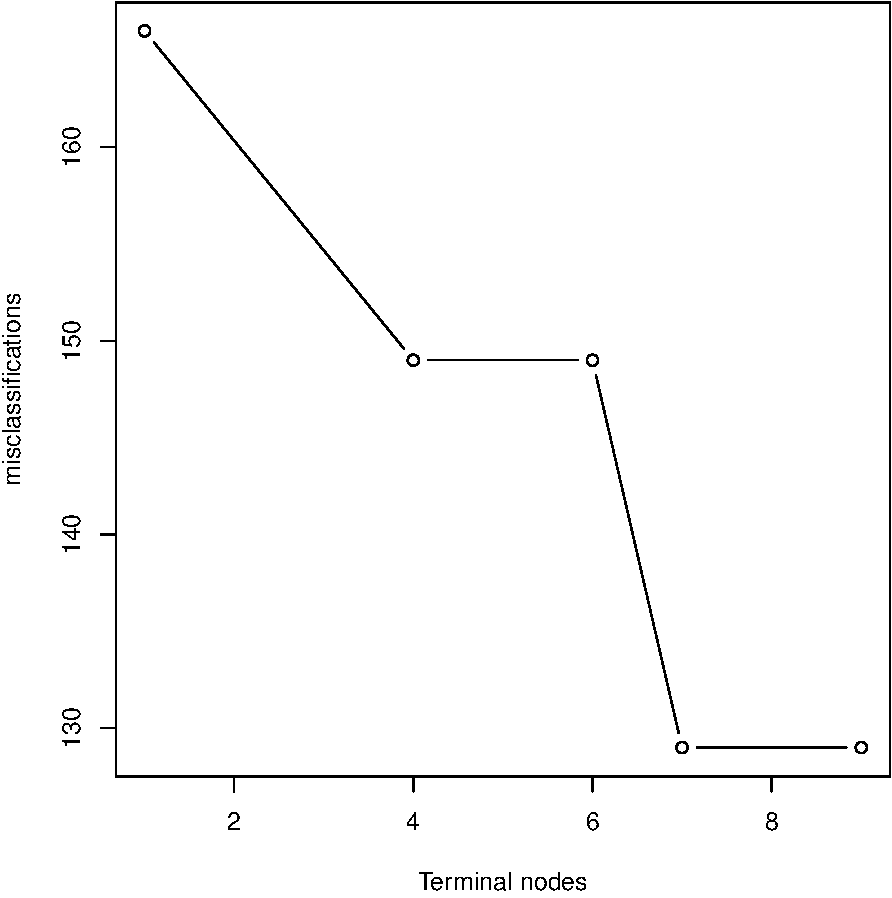
\includegraphics[width=0.7\linewidth]{9TreeBoosting_files/figure-beamer/unnamed-chunk-12-1} \end{center}

\begin{verbatim}
## [1] 1168
\end{verbatim}
\end{frame}

\begin{frame}
\begin{block}{Stochastic GBMs (regularization strategy 3)}
\protect\hypertarget{stochastic-gbms-regularization-strategy-3}{}
\scriptsize

See Boehmke and Greenwell (2020)

\(~\) \normalsize

\begin{itemize}
\tightlist
\item
  Stochastic gradient boosting: chose a random subsample of the training
  data for building each tree (J. H. Friedman 2002).
\end{itemize}

\vspace{2mm}

\begin{itemize}
\tightlist
\item
  Typical value for the proportion \(\eta\) is \(N/2\), but can be much
  smaller when \(N\) is large.
\end{itemize}

\vspace{2mm}

\begin{itemize}
\tightlist
\item
  Again, the idea is to \emph{reduce variance}.
\end{itemize}

\vspace{2mm}

\begin{itemize}
\tightlist
\item
  In addition: Reduction of computation time!
\end{itemize}

\(~\)

\(~\)

\(\rightarrow\) The proportion \(\eta\) is \emph{another
hyper-parameter} that can be tuned\ldots{}
\end{block}
\end{frame}

\begin{frame}[fragile]
\begin{block}{Variants of stochastic GBMs}
\protect\hypertarget{variants-of-stochastic-gbms}{}
\(~\)

There are a few variants of stochastic gradient boosting that can be
used, all of which have additional hyperparameters:

\vspace{2mm}

\begin{itemize}
\tightlist
\item
  Subsample rows before creating each tree
\end{itemize}

\vspace{2mm}

\begin{itemize}
\tightlist
\item
  Subsample columns before creating each tree
\end{itemize}

\vspace{2mm}

\begin{itemize}
\tightlist
\item
  Subsample columns before considering each split in each tree
\end{itemize}

\(~\)

\(~\)

Here we only look at the case where we subsample rows (i.e., entire data
samples), which is available in the \texttt{gbm()} package.
\end{block}
\end{frame}

\begin{frame}[fragile]
We use \texttt{bag.fraction=0.5} to subsample 50\% of the rows each time
we build a tree: \vspace{2mm}

\scriptsize

\begin{Shaded}
\begin{Highlighting}[]
\FunctionTok{set.seed}\NormalTok{(}\DecValTok{123}\NormalTok{)  }\CommentTok{\# for reproducibility}
\NormalTok{ames\_gbm2 }\OtherTok{\textless{}{-}} \FunctionTok{gbm}\NormalTok{(}
  \AttributeTok{formula =}\NormalTok{ Sale\_Price }\SpecialCharTok{\textasciitilde{}}\NormalTok{ .,}
  \AttributeTok{data =}\NormalTok{ ames\_train,}
  \AttributeTok{distribution =} \StringTok{"gaussian"}\NormalTok{,  }\CommentTok{\# SSE loss function}
  \AttributeTok{n.trees =} \DecValTok{3000}\NormalTok{,}
  \AttributeTok{shrinkage =} \FloatTok{0.1}\NormalTok{, }\CommentTok{\# learning rate}
  \AttributeTok{interaction.depth =} \DecValTok{3}\NormalTok{,}
  \AttributeTok{n.minobsinnode =} \DecValTok{10}\NormalTok{, }\CommentTok{\# minimual number of observations in terminal nodes}
  \AttributeTok{cv.folds =} \DecValTok{10}\NormalTok{,}
  \AttributeTok{bag.fraction=}\FloatTok{0.5}
\NormalTok{)}
\end{Highlighting}
\end{Shaded}

\normalsize

Same as before:

\vspace{2mm}

\scriptsize

\begin{Shaded}
\begin{Highlighting}[]
\NormalTok{(best2 }\OtherTok{\textless{}{-}} \FunctionTok{which.min}\NormalTok{(ames\_gbm2}\SpecialCharTok{$}\NormalTok{cv.error))}
\end{Highlighting}
\end{Shaded}

\begin{verbatim}
## [1] 1119
\end{verbatim}

\begin{Shaded}
\begin{Highlighting}[]
\FunctionTok{sqrt}\NormalTok{(ames\_gbm2}\SpecialCharTok{$}\NormalTok{cv.error[best2])}
\end{Highlighting}
\end{Shaded}

\begin{verbatim}
## [1] 22402.07
\end{verbatim}
\end{frame}

\begin{frame}[fragile]{XGBoost: Extreme Gradient Boosting}
\protect\hypertarget{xgboost-extreme-gradient-boosting}{}
Suggested by Chen and Guestrin (2016) and implemented in the R package
\texttt{xgboost}.

\(~\)

\begin{itemize}
\tightlist
\item
  XGBoost is the state-of-the-art for tree boosting and the basis for
  many competition-wining approaches, see for example Kaggle
  competitions (\texttt{https://www.kaggle.com/}).
\end{itemize}

\vspace{2mm}

\begin{itemize}
\tightlist
\item
  It combines many tricks into a very efficient toolbox:
  Parallelization, smart approximations, shrinkage, sub-sampling, etc.
\end{itemize}
\end{frame}

\begin{frame}
Core ideas of XGBoost:

\begin{itemize}
\item
  \emph{\textcolor{red}{Second-order gradients}}: Replace pure first
  order gradient boosting by a second-order (Taylor series) expansion.
\item
  \emph{\textcolor{red}{Parallelization}}: The model is implemented to
  train with multiple CPU cores. Finding new branches is the part that
  is parallelized. Different cores search in different areas of the
  data.
\item
  \emph{\textcolor{red}{Approximation}} of the greedy algorithm for each
  tree by not checking each possible split.
\item
  \emph{\textcolor{red}{Regularization}}: XGBoost includes different
  regularization penalties to avoid overfitting. Each new tree is
  regularized with two terms: The number of leafs (pruning) and the
  weights on the leafs. The total penalizing term is typically given by
  \[\Omega(f) = \gamma |T| + \frac{1}{2}\lambda||w||^2  \text{ (L2 regularization)} \]
  or
  \[\Omega(f) = \gamma |T| +  \alpha ||w|| \text{ (L1 regularization)}  \ .  \]
\end{itemize}
\end{frame}

\begin{frame}
\begin{block}{Some words on regularization in XGBoost}
\protect\hypertarget{some-words-on-regularization-in-xgboost}{}
\(~\)

Previous slide:

\vspace{2mm}

\begin{itemize}
\tightlist
\item
  Pruning parameter \(\gamma\): the new tree is grown to the specified
  depth, and then pruned to find and remove splits according to the
  contraint imposed by \(\gamma\).
\end{itemize}

\vspace{2mm}

\begin{itemize}
\tightlist
\item
  \(\lambda\) and \(\alpha\): Constrain model complexity in the same way
  as ridge or Lasso (L2 and L1).
\end{itemize}

\vspace{4mm}

Additional regularization:

\vspace{2mm}

\begin{itemize}
\tightlist
\item
  The learning rate \(\nu\).
\end{itemize}

\vspace{3mm}

\begin{itemize}
\tightlist
\item
  \emph{Dropout}: Randomly drop trees to avoid that the first trees
  dominate the result.
\end{itemize}

\vspace{3mm}

All these lead to additional hyperparameters.
\end{block}
\end{frame}

\begin{frame}[fragile]
\begin{block}{Ames house pricing example continued}
\protect\hypertarget{ames-house-pricing-example-continued}{}
\vspace{2mm}

We apply XGBoost via the \texttt{xgboost} library on the same dataset as
before. Start by some data preparation:

\(~\)

\scriptsize

\begin{Shaded}
\begin{Highlighting}[]
\FunctionTok{library}\NormalTok{(xgboost)}
\FunctionTok{library}\NormalTok{(recipes)}
 
\CommentTok{\# Training data and response}
\NormalTok{xgb\_prep }\OtherTok{\textless{}{-}} \FunctionTok{recipe}\NormalTok{(Sale\_Price }\SpecialCharTok{\textasciitilde{}}\NormalTok{ ., }\AttributeTok{data =}\NormalTok{ ames\_train) }\SpecialCharTok{\%\textgreater{}\%}
  \FunctionTok{step\_integer}\NormalTok{(}\FunctionTok{all\_nominal}\NormalTok{()) }\SpecialCharTok{\%\textgreater{}\%}
  \FunctionTok{prep}\NormalTok{(}\AttributeTok{training =}\NormalTok{ ames\_train, }\AttributeTok{retain =} \ConstantTok{TRUE}\NormalTok{) }\SpecialCharTok{\%\textgreater{}\%}
  \FunctionTok{juice}\NormalTok{()}

\NormalTok{X }\OtherTok{\textless{}{-}} \FunctionTok{as.matrix}\NormalTok{(xgb\_prep[}\FunctionTok{setdiff}\NormalTok{(}\FunctionTok{names}\NormalTok{(xgb\_prep), }\StringTok{"Sale\_Price"}\NormalTok{)])}
\NormalTok{Y }\OtherTok{\textless{}{-}}\NormalTok{ xgb\_prep}\SpecialCharTok{$}\NormalTok{Sale\_Price}

\CommentTok{\# Test data and test response}
\NormalTok{xgb\_prep\_test }\OtherTok{\textless{}{-}} \FunctionTok{recipe}\NormalTok{(Sale\_Price }\SpecialCharTok{\textasciitilde{}}\NormalTok{ ., }\AttributeTok{data =}\NormalTok{ ames\_test) }\SpecialCharTok{\%\textgreater{}\%}
  \FunctionTok{step\_integer}\NormalTok{(}\FunctionTok{all\_nominal}\NormalTok{()) }\SpecialCharTok{\%\textgreater{}\%}
  \FunctionTok{prep}\NormalTok{(}\AttributeTok{training =}\NormalTok{ ames\_test, }\AttributeTok{retain =} \ConstantTok{TRUE}\NormalTok{) }\SpecialCharTok{\%\textgreater{}\%}
  \FunctionTok{juice}\NormalTok{()}
\NormalTok{X\_test }\OtherTok{\textless{}{-}} \FunctionTok{as.matrix}\NormalTok{(xgb\_prep\_test[}\FunctionTok{setdiff}\NormalTok{(}\FunctionTok{names}\NormalTok{(xgb\_prep\_test), }\StringTok{"Sale\_Price"}\NormalTok{)])}
\NormalTok{Y\_test }\OtherTok{\textless{}{-}}\NormalTok{ xgb\_prep\_test}\SpecialCharTok{$}\NormalTok{Sale\_Price}
\end{Highlighting}
\end{Shaded}
\end{block}
\end{frame}

\begin{frame}[fragile]
Run on training data with a set of hyperparameters that were
pre-optimized\footnote{Adapted from https://bradleyboehmke.github.io/HOML/gbm.html}

\(~\)

\scriptsize

\begin{Shaded}
\begin{Highlighting}[]
\FunctionTok{set.seed}\NormalTok{(}\DecValTok{123}\NormalTok{)}
\NormalTok{ames\_xgb }\OtherTok{\textless{}{-}} \FunctionTok{xgboost}\NormalTok{(}
  \AttributeTok{data =}\NormalTok{ X,}
  \AttributeTok{label =}\NormalTok{ Y,}
  \AttributeTok{nrounds =} \DecValTok{6000}\NormalTok{,}
  \AttributeTok{objective =} \StringTok{"reg:squarederror"}\NormalTok{,}
  \AttributeTok{early\_stopping\_rounds =} \DecValTok{50}\NormalTok{,   }
  
  \AttributeTok{params =} \FunctionTok{list}\NormalTok{( }
    \AttributeTok{eta =} \FloatTok{0.1}\NormalTok{, }\CommentTok{\# learning rate (nu)}
    \AttributeTok{lambda=}\FloatTok{0.01}\NormalTok{, }\CommentTok{\# L2 regularization term}
    \AttributeTok{max\_depth =} \DecValTok{3}\NormalTok{,}
    \AttributeTok{min\_child\_weight =} \DecValTok{3}\NormalTok{,}
    \AttributeTok{subsample =} \FloatTok{0.8}\NormalTok{, }\CommentTok{\# Proportion of datapoints used for each tree}
    \AttributeTok{colsample\_bytree =} \FloatTok{0.5}\NormalTok{, }\CommentTok{\# subsample ratio of columns when constructing each tree}
    \AttributeTok{nthread=}\DecValTok{12}\NormalTok{),}
  \AttributeTok{verbose =} \DecValTok{0}
\NormalTok{)  }
\end{Highlighting}
\end{Shaded}

\begin{Shaded}
\begin{Highlighting}[]
\NormalTok{X.pred.test }\OtherTok{\textless{}{-}} \FunctionTok{predict}\NormalTok{(ames\_xgb,}\AttributeTok{newdata =}\NormalTok{ X\_test)}
\FunctionTok{sqrt}\NormalTok{(}\FunctionTok{sum}\NormalTok{((X.pred.test }\SpecialCharTok{{-}}\NormalTok{ Y\_test)}\SpecialCharTok{\^{}}\DecValTok{2}\NormalTok{)}\SpecialCharTok{/}\FunctionTok{nrow}\NormalTok{(X\_test))}
\end{Highlighting}
\end{Shaded}

\begin{verbatim}
## [1] 19935.63
\end{verbatim}
\end{frame}

\begin{frame}
\begin{block}{Hyperparameter tuning}
\protect\hypertarget{hyperparameter-tuning}{}
\(~\)

\begin{itemize}
\tightlist
\item
  Hyperparameters in many dimensions.
\end{itemize}

\vspace{2mm}

\begin{itemize}
\tightlist
\item
  Tuning the models becomes very slow! We refer to Boehmke and Greenwell
  (2020) for parameter tuning runs:\\
  \url{https://bradleyboehmke.github.io/HOML/gbm.html}
\end{itemize}

\vspace{2mm}

\begin{itemize}
\tightlist
\item
  See exercise session.
\end{itemize}
\end{block}
\end{frame}

\begin{frame}{Most recent advances: LightBGM, CatBoost}
\protect\hypertarget{most-recent-advances-lightbgm-catboost}{}
From \url{https://bradleyboehmke.github.io/HOML/gbm.html}:

\begin{itemize}
\item
  LightGBM (Ke et al.~2017) is a gradient boosting framework that
  focuses on leaf-wise tree growth versus the traditional level-wise
  tree growth. This means as a tree is grown deeper, it focuses on
  extending a single branch versus growing multiple branches
\item
  CatBoost (Dorogush, Ershov, and Gulin 2018) is another gradient
  boosting framework that focuses on using efficient methods for
  encoding categorical features during the gradient boosting process.
\end{itemize}

Both frameworks are available in R.
\end{frame}

\begin{frame}{Interpretation of tree ensembles}
\protect\hypertarget{interpretation-of-tree-ensembles}{}
\(~\)

\begin{itemize}
\tightlist
\item
  Single trees are easy to interpret.
\end{itemize}

\vspace{2mm}

\begin{itemize}
\tightlist
\item
  Tree ensembles or linear combinations of trees (like in boosting)
  sacrifice interpretability.
\end{itemize}

\vspace{2mm}

\begin{itemize}
\tightlist
\item
  In Module 8 we have heard about \emph{relative importance of predictor
  variables}.
\end{itemize}

\vspace{2mm}

\begin{itemize}
\tightlist
\item
  Another way to gain interpretability back is via
  \emph{\textcolor{red}{partial dependence plots}}. They show the effect
  of individual predictors, where the effect of the other predictor
  variables is integrated out (see Hastie, Tibshirani, and Friedman
  (2009), Section 10.13.2).
\end{itemize}
\end{frame}

\begin{frame}
\begin{block}{Partial dependence plots}
\protect\hypertarget{partial-dependence-plots}{}
\scriptsize

(Section 10.13.2 in the Elements book Hastie, Tibshirani, and Friedman
(2009))

\normalsize

\(~\)

\begin{itemize}
\tightlist
\item
  Motivation: We would like to have a \emph{qualitative description} of
  how a single variable affects the response.
\end{itemize}

\vspace{3mm}

\begin{itemize}
\tightlist
\item
  Partial dependence plots provide such a description. They can be used
  to interpret results from any ``black box'' method.
\end{itemize}

\vspace{3mm}

\begin{itemize}
\tightlist
\item
  For input variable \(X_j\), the \emph{partial dependence} of \(f(X)\)
  on \(X_j\) is given as \[\text{E}_{X_j} f(X_j, X_{-j}) \ , \] where
  \(X_{-j}\) denotes the set of all variables \emph{except} \(X_j\).
\end{itemize}
\end{block}
\end{frame}

\begin{frame}
\vspace{2mm}

\begin{itemize}
\tightlist
\item
  For boosted trees, we estimate the partial dependence by taking the
  average over all observations
  \[\overline{f}(X_j) = \frac1N \sum_{i=1}^N f(X_{j},(X_{-j})_i)\] for a
  set of values for \(X_j\), where we evaluate the estimated tree value
  \(f(X_{j},(X_{-j})_i\) for each data point \(i\).
\end{itemize}

\vspace{4mm}

\begin{itemize}
\tightlist
\item
  Note: The partial dependence function represents the effects of
  \(X_j\) on \(f(X)\) \emph{after} accounting for the effects of the
  other variables. They are not the effects of \(X_j\) on \(f(X)\)
  independent of the other variables!
\end{itemize}

\normalsize
\end{frame}

\begin{frame}[fragile]
\begin{block}{Partial dependence plots for the Boston example}
\protect\hypertarget{partial-dependence-plots-for-the-boston-example}{}
\(~\)

\texttt{rm} (number of rooms) and \texttt{lstat} (\% of lower status
population) are the most important predictors.

\vspace{2mm}

\scriptsize

\begin{Shaded}
\begin{Highlighting}[]
\FunctionTok{plot}\NormalTok{(boost.boston,}\AttributeTok{i=}\StringTok{"rm"}\NormalTok{,}\AttributeTok{ylab=}\StringTok{"medv"}\NormalTok{)}
\end{Highlighting}
\end{Shaded}

\begin{center}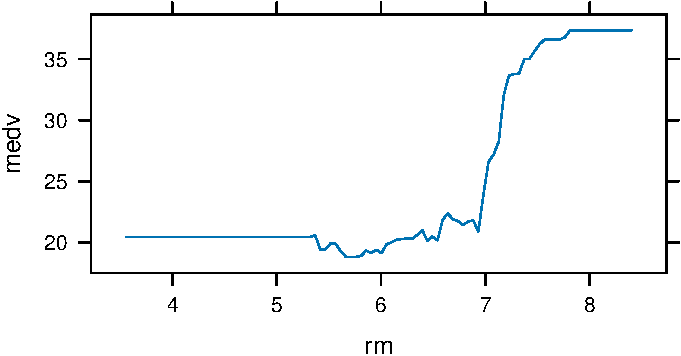
\includegraphics[width=0.4\linewidth]{9TreeBoosting_files/figure-beamer/boston7-1} \end{center}

\begin{Shaded}
\begin{Highlighting}[]
\FunctionTok{plot}\NormalTok{(boost.boston,}\AttributeTok{i=}\StringTok{"lstat"}\NormalTok{,}\AttributeTok{ylab=}\StringTok{"medv"}\NormalTok{)}
\end{Highlighting}
\end{Shaded}

\begin{center}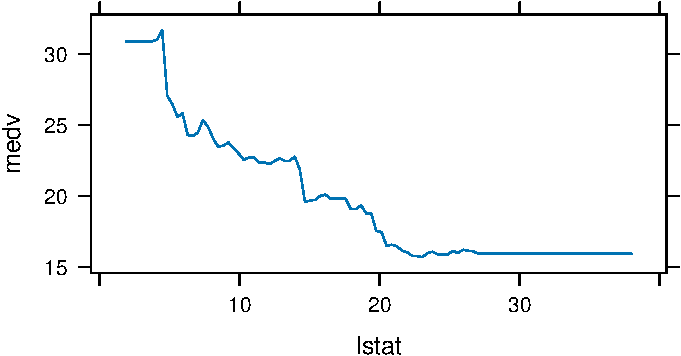
\includegraphics[width=0.4\linewidth]{9TreeBoosting_files/figure-beamer/boston7-2} \end{center}
\end{block}
\end{frame}

\begin{frame}{Can we use boosting for linear regression models?}
\protect\hypertarget{can-we-use-boosting-for-linear-regression-models}{}
\(~\)

Yes!

Didrik Lindløv Sand, a current master student, will present his work.
\end{frame}

\begin{frame}{References}
\protect\hypertarget{references}{}
\tiny

\hypertarget{refs}{}
\begin{CSLReferences}{1}{0}
\leavevmode\vadjust pre{\hypertarget{ref-boehmke_greenwell2020}{}}%
Boehmke, B., and B. Greenwell. 2020. \emph{Hands-on Machine Learning
with {R}}. https://bradleyboehmke.github.io/HOML/: CRC press.

\leavevmode\vadjust pre{\hypertarget{ref-chen2016xgboost}{}}%
Chen, Tianqi, and Carlos Guestrin. 2016. {``Xgboost: A Scalable Tree
Boosting System.''} In \emph{Proceedings of the 22nd Acm Sigkdd
International Conference on Knowledge Discovery and Data Mining},
785--94.

\leavevmode\vadjust pre{\hypertarget{ref-freund1997decision}{}}%
Freund, Yoav, and Robert E Schapire. 1997. {``A Decision-Theoretic
Generalization of on-Line Learning and an Application to Boosting.''}
\emph{Journal of Computer and System Sciences} 55 (1): 119--39.

\leavevmode\vadjust pre{\hypertarget{ref-friedman2002}{}}%
Friedman, Jerome H. 2002. {``Stochastic Gradient Boosting.''}
\emph{Computational Statistics \& Data Analysis} 38: 367--78.

\leavevmode\vadjust pre{\hypertarget{ref-friedman2000additive}{}}%
Friedman, Jerome, Trevor Hastie, and Robert Tibshirani. 2000.
{``Additive Logistic Regression: A Statistical View of Boosting (with
Discussion and a Rejoinder by the Authors).''} \emph{The Annals of
Statistics} 28 (2): 337--407.

\leavevmode\vadjust pre{\hypertarget{ref-hastie_etal2009}{}}%
Hastie, Trevor, Robert Tibshirani, and Jerome Friedman. 2009. \emph{The
Elements of Statistical Learning}. Vol. 2. Springer series in statistics
New York.

\leavevmode\vadjust pre{\hypertarget{ref-ISL2}{}}%
James, Gareth, Daniela Witten, Trevor Hastie, and Robert Tibshirani.
2021. \emph{An Introduction to Statistical Learning}. 2nd ed. Vol. 112.
Springer.

\leavevmode\vadjust pre{\hypertarget{ref-ridgeway1999state}{}}%
Ridgeway, Greg. 1999. {``The State of Boosting.''} \emph{Computing
Science and Statistics}, 172--81.

\end{CSLReferences}
\end{frame}

\end{document}
